
% \eqref{sep/2/7/eq:parab} can be written as
% \begin{align}
% y^2 - x &= 0
% \label{sep/2/7/eq:parab_twovar}
% \end{align}

The matrix parameters  for the given curve are
\begin{align}
\vec{V} = \myvec{0 & 0\\0 & 1}, \vec{u} = \myvec{\frac{-1}{2}\\0}, \vec{f}=0.
\label{sep/2/7/eq:parab_twovar_params}
\end{align}
Thus, the given curve is a parabola.  $\because \vec{V}$ is diagonal and in standard form,
\begin{align}
\vec{V}\vec{p} &= \vec{0}
\\
\implies \vec{p} &= \myvec{1\\0}
\label{sep/2/7/eq:parab_twovar_p}
\end{align}
with eigen parameters
\begin{align}
\lambda_1=0, \lambda_2=1
\end{align}
The line   $x=1$  can be expressed as
\begin{align}
\vec{x}=\myvec{1\\0}+\vec{y}\myvec{0\\1}\\
\myvec{1 & 0}\vec{x}=\myvec{1 & 0}\myvec{1\\0}+\vec{y}\myvec{1 & 0}\myvec{0\\1}\\
\myvec{1 & 0}\vec{x}=1\label{sep/2/7/eq:line1}
\end{align}
Similarly, for ${x}=4$ we get
\begin{align}\label{sep/2/7/eq:line2}
\myvec{4 & 0}\vec{x}=16\\
\implies\myvec{1 & 0}\vec{x}=4
\end{align}
The direction vector and normal vectors are
\begin{align}
\vec{m} = \myvec{0\\1}, \vec{n} = \myvec{1\\0}.
\label{sep/2/7/eq:parab_twovar_mn}
\end{align}
The equation of parabola is
\begin{align}
\vec{q}^T\vec{V}\vec{q} + 2\vec{u}^T\vec{q} +f = 0
\label{sep/2/7/eq:conic_tangent_qquad}
\end{align}\\
The vertex of conic section in \eqref{sep/2/7/eq:conic_tangent_qquad} is given by $\vec{c}$ using  
\begin{align}
\label{sep/2/7/eq:vertex}
\begin{pmatrix}
\vec{u^T+n \vec{p}}^T \\ \vec{V}
\end{pmatrix}
\vec{c} &= 
\begin{pmatrix}
-f
\\
\vec{n}\vec{p}-\vec{u}
\end{pmatrix}
\end{align}
\begin{align}
\myvec{\frac{-1}{4} & 0 \\ 0 & 0 \\ 0 & 1}\vec{c} &= \myvec{0 \\ 0\\0} 
\\
\implies 
\myvec{\frac{-1}{4} & 0 \\  0 & 1}\vec{c} &= \myvec{0 \\ 0} 
\\
\text{or, } \vec{c} = \myvec{0\\0}
\end{align}
\begin{align}
\label{sep/2/7/eq:conic_tangent_qk_eigen} \kappa = \frac{\vec{p}_1^T\vec{u}}{\vec{p}_1^T\vec{n}}, \quad 
\end{align}
From \eqref{sep/2/7/eq:conic_tangent_qk_eigen}, \eqref{sep/2/7/eq:parab_twovar_mn} and \eqref{sep/2/7/eq:parab_twovar_p},
\begin{align}
\kappa =\frac{-1}{2}
\end{align}
which, upon substitution in  \eqref{sep/2/7/eq:conic_tangent_q_eigen}
\begin{align}
\label{sep/2/7/eq:conic_tangent_q_eigen}
\begin{pmatrix}
\vec{u+\kappa \vec{n}}^T \\ \vec{V}
\end{pmatrix}
\vec{q} &= 
\begin{pmatrix}
-f
\\
\kappa\vec{n}-\vec{u}
\end{pmatrix}
\end{align}
and simplification yields the matrix equation
\begin{align}
\myvec{\frac{-1}{2} & 0 \\0 & 0\\0&1}\vec{q} &= \myvec{0\\0\\0}
\\
\implies \myvec{\frac{-1}{2} & 0\\0&1}\vec{q} &= \myvec{0\\0}
\\
\text{or, } \vec{q} &= \myvec{0 \\0}
\end{align}
 
{\em Secant: }The points of intersection of the line 
\begin{align}
L: \quad \vec{x} = \vec{q} + \mu \vec{m} \quad \mu \in \mathbb{R}
\label{sep/2/7/eq:conic_tangent}
\end{align}
\begin{align}\label{sep/2/7/eq:parametricform}
\vec{x}_i = \vec{q} + \mu_i \vec{m}
\end{align}
%
where
\begin{multline}
\mu_i = \frac{1}
{
\vec{m}^T\vec{V}\vec{m}
}
\lbrak{-\vec{m}^T\brak{\vec{V}\vec{q}+\vec{u}}}
\\
\pm
{\small
\rbrak{\sqrt{
\sbrak{
\vec{m}^T\brak{\vec{V}\vec{q}+\vec{u}}
}^2
-
\brak
{
\vec{q}^T\vec{V}\vec{q} + 2\vec{u}^T\vec{q} +f
}
\brak{\vec{m}^T\vec{V}\vec{m}}
}
}
}
\label{sep/2/7/eq:tangent_roots}
\end{multline}
                    
$\because \vec{q}$ is the point of contact, $\vec{q}$ satisfies parabola equation

 
Given the point of contact $\vec{q}$, the equation of a tangent is 
\begin{align}
\brak{\vec{V}\vec{q}+\vec{u}}^T\vec{x}+\vec{u}^T\vec{q}+f = 0
\label{sep/2/7/eq:conic_tangent_final}
\end{align}
%
From \eqref{sep/2/7/eq:tangent_roots} we get 
$\mu_1= 1, \mu_2= -1$

The lines \eqref{sep/2/7/eq:line1}, \eqref{sep/2/7/eq:line2} can be written in parametric form in \eqref{sep/2/7/eq:parametricform} we get
\begin{align}\label{sep/2/7/eq:para1}
\vec{x}_i = \myvec{ 1\\ 0} + \mu_i \myvec{0\\1}
\end{align}
Substituting $\mu_1, \mu_2$ value in \eqref{sep/2/7/eq:para1} we get

\begin{align}
\vec{x}_i = \myvec{1\\0} + 1\myvec{0\\1}\\
\implies\vec{K_1}=\myvec{1\\1}
\end{align}
\begin{align}
\vec{x}_i = \myvec{1\\0} + -1\myvec{0\\1}\\
\implies\vec{L_1}=\myvec{1\\-1}
\end{align}
For $x= 4$, 
\begin{align}\label{sep/2/7/eq:para2}
\vec{x}_i = \myvec{ 4\\ 0} + \mu_i \myvec{0\\1}
\end{align}
\begin{align}
\vec{x}_i = \myvec{4\\0} + 2\myvec{0\\1}\\
\implies\vec{K_2}=\myvec{4\\2}
\end{align}
\begin{align}
\vec{x}_i = \myvec{4\\0} + -2\myvec{0\\1}\\
\implies\vec{L_2}=\myvec{4\\-2}
\end{align}
The area enclosed by parabola and line on x-axis can be given as
A = Area under line - Area under curve
\begin{align}
\implies\boxed{\vec{A} = \vec{A_1}-\vec{A_3}} \label{sep/2/7/eq:A}
\end{align}
%
Performing integration,
% Area under the parabola\eqref{sep/2/7/eq:parab} i.e,

% \vec{A} =$\int$\vec{x}^\frac{1}{2} dx \\

In Fig. \ref{sep/2/7/fig:parab_tangent}	, the  area under the lines \eqref{sep/2/7/eq:line1}, \eqref{sep/2/7/eq:line2} is given by
\begin{align}
\vec{A_1} =\frac{2}{3},
\vec{A_2}=\frac{16}{3}  
\end{align}
Putting these values in \eqref{sep/2/7/eq:A} we get
\begin{align}
\implies\boxed{\vec{A} =\frac{14}{3}}
\end{align}
%
\begin{figure}[!ht]
\centering
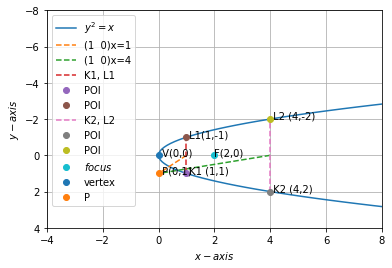
\includegraphics[width=\columnwidth]{solutions/sep/2/7/download.png}
\caption{Parabola $\vec{y^2} = \vec{x}$ }
\label{sep/2/7/fig:parab_tangent}	
\end{figure}


